\documentclass{article}
\usepackage{listings}
\usepackage{xcolor}
\usepackage{ctex,graphicx}

\begin{document}

\section*{第一题}
\subsection{运行结果}
\label{subsec:label}
\textbf{注意左边图片是生产者,右边图片时消费者}\\
\textbf{参数为(1,1)时结果---分别对应生产者,消费者}\\
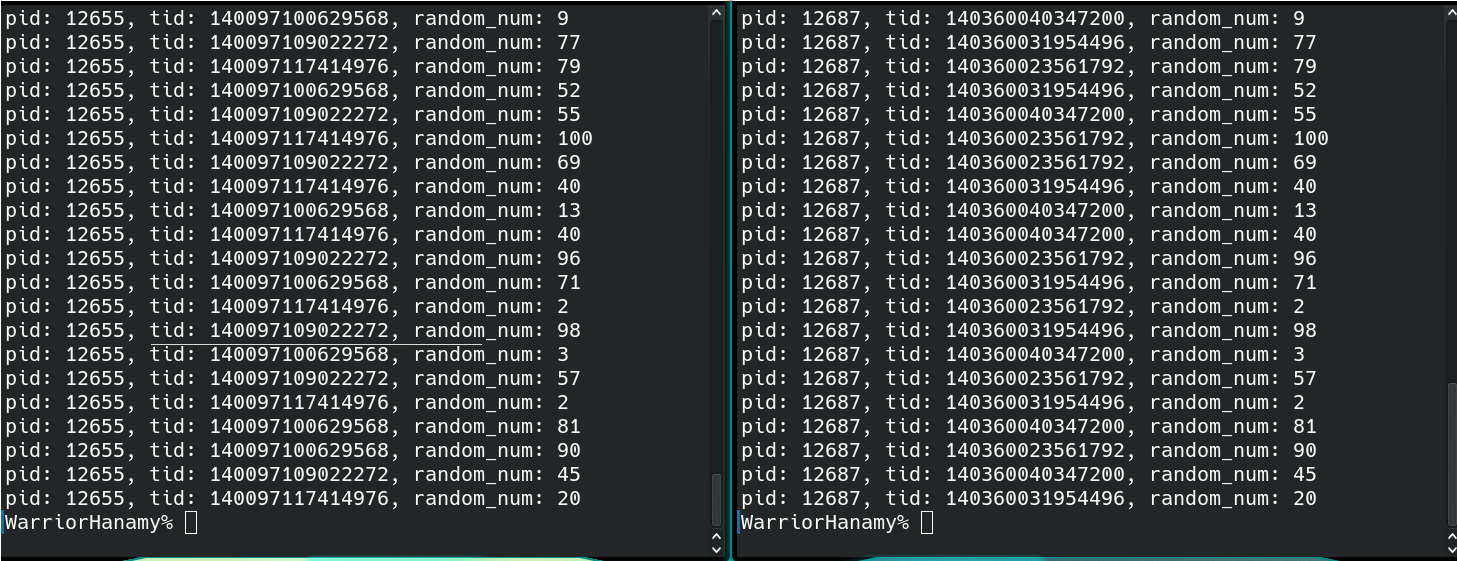
\includegraphics[scale=0.35]{11.png}
\textbf{参数为(1,2)时结果,生产速度快于消费速度}\\
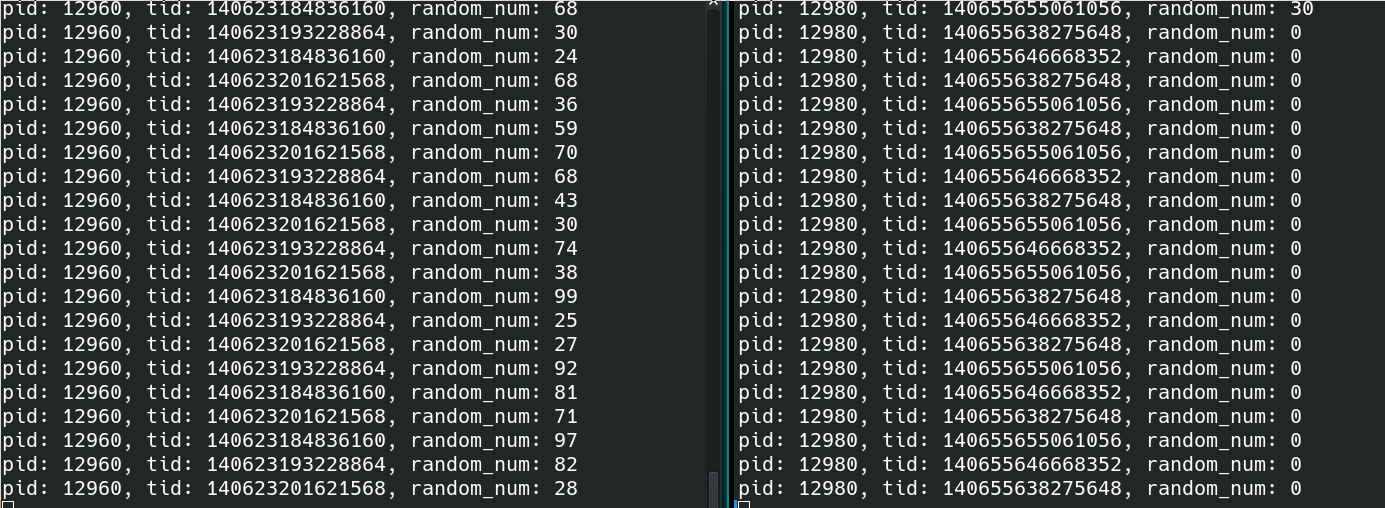
\includegraphics[scale=0.35]{12.png}
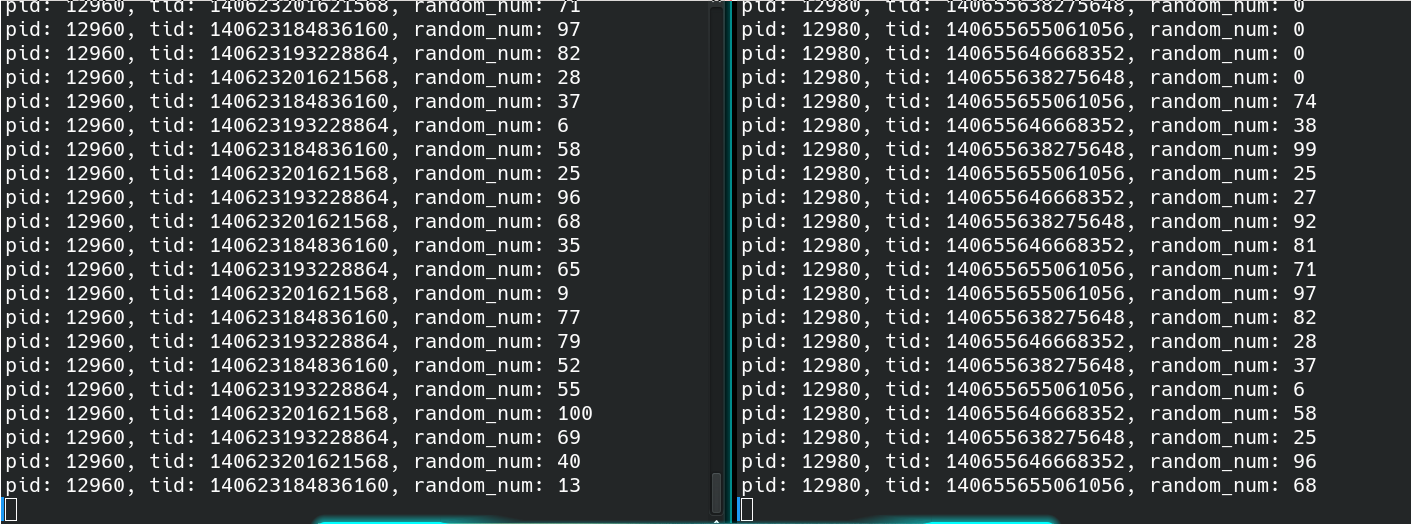
\includegraphics[scale=0.35]{12-2.png}
\textbf{参数为(2,1)时结果,生产速度小于消费速度}\\
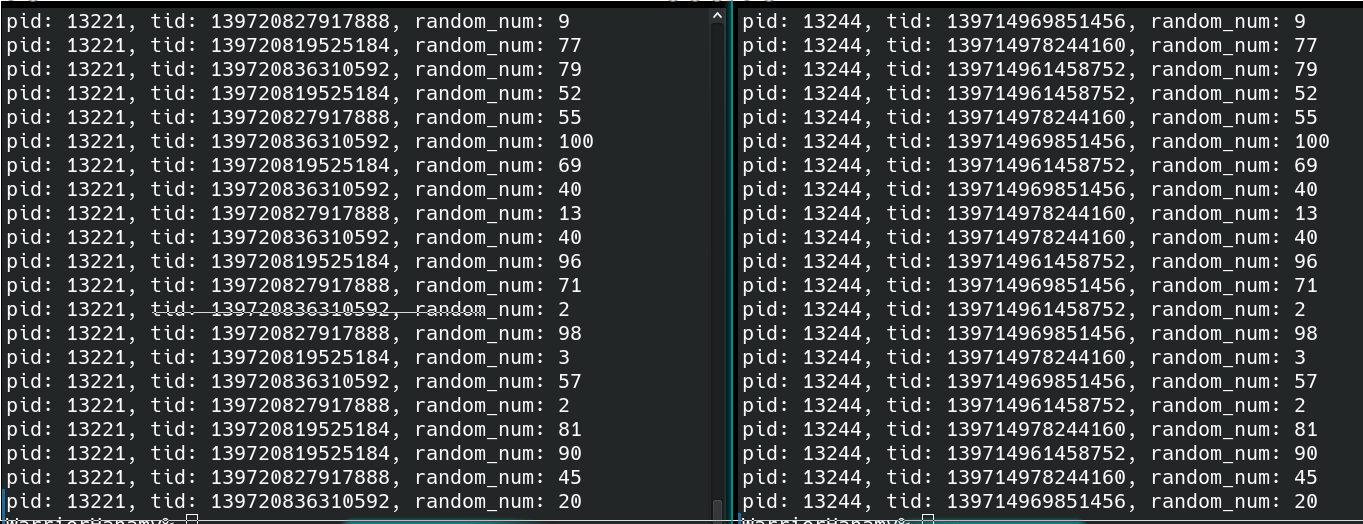
\includegraphics[scale=0.35]{21.png}
\subsection{生产者代码部分}
\label{subsec:label}

\lstset{language=C}
\begin{lstlisting}
#include <stdio.h>
#include <string.h>
#include <fcntl.h>
#include <sys/stat.h>
#include <semaphore.h>
#include <unistd.h>
#include <stdlib.h>
#include <sys/mman.h>
#include <time.h>
#include <math.h>
#include <pthread.h>

/// BASIC STRUCTURE
#define NUM_THREADS 3
#define MAX_PRODUCT 20
typedef struct product_s
{
	pthread_mutex_t mutex;
	short init;
	int rear;
	int front;
	int data[20];
}product;


int negative_exponential_distribution(double lambda)
{
	double pV = 0.0;
    while(1)
    {
        pV = (double)rand()/(double)RAND_MAX;
        if (pV != 1)
        {
            break;
        }
    }
    pV = (-1.0/lambda)*log(1-pV);
    return (int)(pV * 1000000);
}

sem_t *sem_full;
sem_t *sem_empty;
product *p;
pthread_t tid[NUM_THREADS];

void *producer(void *param)
{
	int lambda = *(int*)param;
	int random_time = negative_exponential_distribution(lambda);
	usleep(random_time);



	int random_data = rand() % 100 + 1;

///CRTICAL REGION///
	sem_wait(sem_empty);
	pthread_mutex_lock(&(p->mutex));
    p->data[p->rear] = random_data;
    printf("pid: %d, tid: %lu, random_num: %d\n",
                      getpid(), (unsigned long)pthread_self(), p->data[p->rear]);
	p->rear = (p->rear + 1) % MAX_PRODUCT;
	pthread_mutex_unlock(&(p->mutex));
    sem_post(sem_full);

}

int main(int argc, char** argv)
{

    sem_full = sem_open("/Full", O_CREAT, 0644, 0);


    sem_empty = sem_open("/Empty", O_CREAT, 0644, 20);

    ///SHARED MEMORY CREATE
    int fd = shm_open("/sh_product", O_CREAT | O_RDWR, 0644);


    ftruncate(fd, sizeof(product));

    //MAP FOR SHARED MOREMORY
    p = mmap(0, sizeof(product), PROT_WRITE, MAP_SHARED, fd, 0);
    p->init = 0;


    if (p->init != 1) {
        memset(p, 0, sizeof(product));
        p->init = 1;
    }

    pthread_mutex_init(&(p->mutex), NULL);


    pthread_attr_t attr;
    pthread_attr_init(&attr);

    int lambda = atoi(argv[1]);

    for (int loop = 0; loop < 20; loop++)
	{
	    int i;
		for(i = 0; i < NUM_THREADS; i++)
	        pthread_create(&tid[i], &attr, producer, &lambda);

	    for(i = 0; i < NUM_THREADS; i++)
	        pthread_join(tid[i], NULL);
	}


    munmap(p, sizeof(product));
    //UNLINK SHARED MOREMORY
    shm_unlink("/sh_product");

    sem_close(sem_full);
    sem_close(sem_empty);

    return 0;
}

\end{lstlisting}

\subsection{消费者代码部分}
\label{subsec:label}


\lstset{language=C}
\begin{lstlisting}
#include <stdio.h>
#include <string.h>
#include <fcntl.h>
#include <sys/stat.h>
#include <semaphore.h>
#include <unistd.h>
#include <stdlib.h>
#include <sys/mman.h>
#include <time.h>
#include <math.h>
#include <pthread.h>

//SAME TO prodocuer.c

///BASIC STRUCTURE
#define NUM_THREADS 3
#define MAX_PRODUCT 20
typedef struct product_s
{
	pthread_mutex_t mutex;
	short init;
	int rear;
	int front;
	int data[20];
}product;

int negative_exponential_distribution(double lambda){
	double pV = 0.0;
    while(1)
    {
        pV = (double)rand()/(double)RAND_MAX;
        if (pV != 1)
        {
            break;
        }
    }
    pV = (-1.0/lambda)*log(1-pV);
    return (int)(pV * 1000000);
}

sem_t *sem_full;
sem_t *sem_empty;
product *p;
pthread_t tid[NUM_THREADS];

void *consumer(void *param)
{
	int lambda = *(int*)param;
	int random_time = negative_exponential_distribution(lambda);
	usleep(random_time);


    sem_wait(sem_full);


    pthread_mutex_unlock(&(p->mutex));
    printf("pid: %d, tid: %lu, random_num: %d\n", getpid(), (unsigned long)pthread_self(), p->data[p->front]);
    p->data[p->front] = 0;
    p->front = (p->front + 1) % MAX_PRODUCT;
	pthread_mutex_unlock(&(p->mutex));

    sem_post(sem_empty);


}

int main(int argc, char** argv)
{

	sem_full = sem_open("/Full", O_EXCL, 0644, 0);
    if (sem_full == SEM_FAILED) {
        fprintf(stderr, "sem_open error\n");
        exit(1);
    }


    sem_empty = sem_open("/Empty", O_EXCL, 0644, 20);
    if (sem_empty == SEM_FAILED) {
        fprintf(stderr, "sem_open error\n");
        exit(1);
    }


    int fd = shm_open("/sh_product", O_CREAT | O_RDWR, 0666);
    if (fd < 0) {
        fprintf(stderr, "shm_open error\n");
        exit(1);
    }


    p = mmap(NULL, sizeof(product), PROT_WRITE, MAP_SHARED, fd, 0);
    if (p == MAP_FAILED) {
        fprintf(stderr, "mmap error\n");
        exit(1);
    }

    if (p->init != 1) {
        memset(p, 0, sizeof(product));
        p->init = 1;
    }

    pthread_attr_t attr;
    pthread_attr_init(&attr);

    int lambda = atoi(argv[1]);
    int loop;
    for (loop = 0; loop < 20; loop++)
	{
	    int i;
		for(i = 0; i < NUM_THREADS; i++)
	        pthread_create(&tid[i], &attr, consumer, &lambda);

	    for(i = 0; i < NUM_THREADS; i++)
	        pthread_join(tid[i], NULL);
	}

    munmap(p, sizeof(product));
    shm_unlink("/sh_product");

    sem_close(sem_full);
    sem_close(sem_empty);

    return 0;
}
\end{lstlisting}




\section*{第二题}
\subsection{运行结果}
\label{subsec:label}

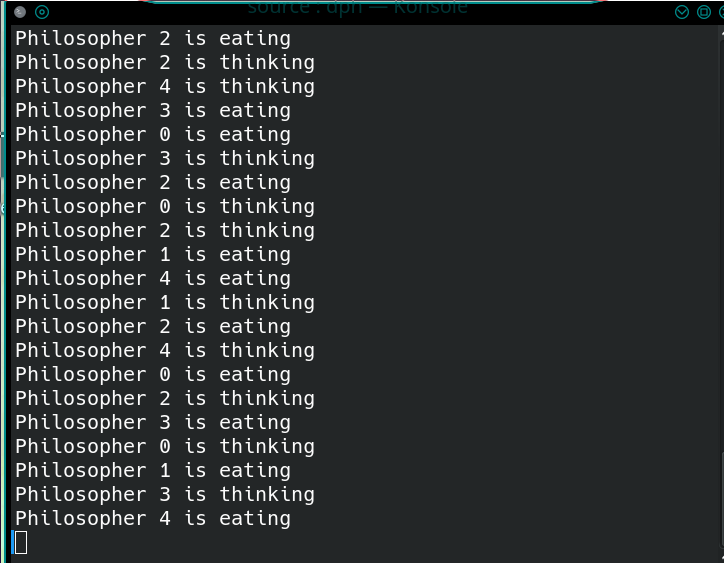
\includegraphics[scale=0.6]{Philosopher.png}


\subsection{哲学家代码部分}
\label{subsec:label}


\lstset{language=C}
\begin{lstlisting}        %插入要显示的代码

#include <pthread.h>
#include <stdio.h>
#include <stdlib.h>
#include <unistd.h>
#include <time.h>
#include <pthread.h>


#define NUMBER 5
#define MAX_SLEEP_TIME	3
enum {THINKING, HUNGRY, EATING} state[NUMBER];

// THREADS FOR PHILOSOPHERS
int thread_id[NUMBER];


pthread_cond_t		cond_vars[NUMBER];
pthread_mutex_t 	mutex_lock;

void *philosopher(void *param);
pthread_t tid[NUMBER];

void init()
{
	int i;

	for (i = 0; i < NUMBER; i++)
	{
		state[i] = THINKING;
		thread_id[i] = i;
		pthread_cond_init(&cond_vars[i],NULL);
	}

	pthread_mutex_init(&mutex_lock, NULL);


	for (i = 0; i < NUMBER; i++)
		pthread_create(&tid[i], 0, philosopher, (void *)&thread_id[i]);
}

void test(int i)
{
	if ( (state[(i + NUMBER - 1) % NUMBER] != EATING) && (state[i] == HUNGRY) && (state[(i + 1) % NUMBER] != EATING) )
	{
		state[i] = EATING;
		printf("Philosopher %d is eating\n", i);
		pthread_cond_signal(&cond_vars[i]);
	}
}

void pickup_forks(int number)
{
	pthread_mutex_lock(&mutex_lock);

	state[number] = HUNGRY;

	test(number);
	while (state[number] != EATING)
		pthread_cond_wait(&cond_vars[number], &mutex_lock);

	pthread_mutex_unlock(&mutex_lock);
}

void return_forks(int number)
{
	pthread_mutex_lock(&mutex_lock);

	state[number] = THINKING;
	printf("Philosopher %d is thinking\n", number);


	test((number + NUMBER - 1) % NUMBER);
	test((number + 1) % NUMBER);

	pthread_mutex_unlock(&mutex_lock);
}

void *philosopher(void *param)
{
	int number = *(int *)param;
	int sleep_time = (rand() % 3) + 1;



	while(1)
	{
		sleep(sleep_time);
		pickup_forks(number);

		sleep(sleep_time);
		return_forks(number);
	}
}

int main()
{
	init();

	int i;
	for (i = 0; i < NUMBER; i++)
		pthread_join(tid[i],NULL);
	return 0;
}

\end{lstlisting}

\section*{第三题}
\subsection{sleep运行结果}
\label{subsec:label}
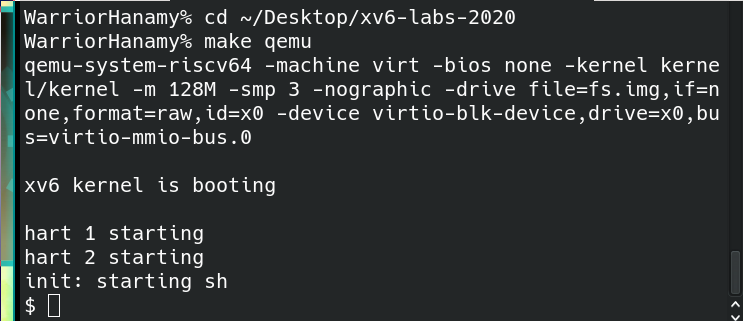
\includegraphics[scale=0.6]{boot.png}
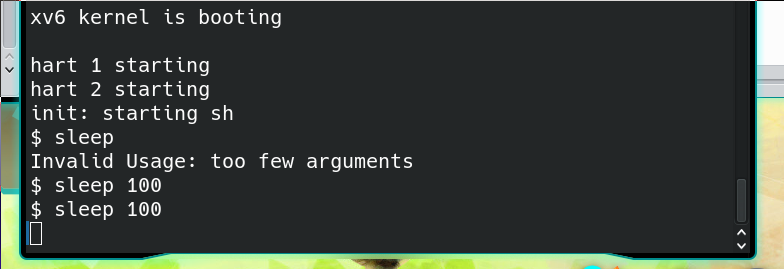
\includegraphics[scale=0.6]{sleep.png}
\subsection{sleep代码部分}
\label{subsec:label}


\lstset{language=C}
\begin{lstlisting}        %插入要显示的代码

#include "kernel/types.h"
#include "user.h"

int main(int argc, char *argv[]) {
	int sleep_sec;
	if (argc < 2){
		printf("Invalid Usage: too few arguments\n");
		exit(1);
	}

	sleep_sec = atoi(argv[1]);
	if (sleep_sec > 0){
		sleep(sleep_sec);
	} else {
		printf("Invalid interval %s\n", argv[1]);
	}
	exit(0);
}
\end{lstlisting}

\subsection{第三题第二部分}
\label{subsec:label}
ddl到了,没写完







\end{document}

%%% Local Variables:
%%% mode: latex
%%% TeX-master: t
%%% End:
